\documentclass[8pt]{article}
\usepackage[UTF8]{ctex}
\usepackage[a4paper]{geometry}

\usepackage{amsthm,amsmath,amssymb}
\usepackage{graphicx}
\usepackage{subfigure}
\usepackage{amsmath}
\usepackage{tabularx}
\usepackage{color}
\usepackage{hyperref}
\usepackage{ulem}
\usepackage{multirow}
\usepackage[cache=false]{minted}
\hypersetup{
	colorlinks=true,
	linkcolor=blue
}

\usepackage{appendix}
\geometry{a4paper,centering,scale=0.8}
\geometry{left=2.0cm, right=2.0cm, top=2.5cm, bottom=2.5cm}
\usepackage[format=hang,font=small,textfont=it]{caption}
\usepackage[nottoc]{tocbibind}

\usepackage{algorithm}
\usepackage{algorithmicx}
\usepackage{algpseudocode}
\usepackage{amssymb}
\usepackage{extarrows}
\usepackage{qcircuit}
\usepackage{fancyhdr}
\usepackage{cleveref}
\usepackage{totpages}
\usepackage{pgf}
\usepackage{tikz}
\usepackage{bbm}
\usetikzlibrary{arrows,automata}
\usetikzlibrary{arrows.meta}%画箭头用的包

\makeatletter
\def\@maketitle{%
	\newpage
	\begin{center}%
		\let \footnote \thanks
		{\LARGE \@title \par}%
		\vskip 1.5em%
		{\large
			\lineskip .5em%
			\begin{tabular}[t]{c}%
				\@author
			\end{tabular}\par}%
		\vskip 1em%
		{\large \@date}%
	\end{center}%
	\par
	\vskip 1.5em}
\makeatother

\newtheoremstyle{compact}%
{3pt}{3pt}%
{}{}%
{\bfseries}{\textcolor{red}{.}}%  % Note that final punctuation is omitted.
{.5em}{\mbox{\textcolor{red}{\thmname{#1}\thmnumber{ #2}}\thmnote{ (\textcolor{blue}{#3})}}}
\theoremstyle{compact}
\newtheorem{innercustomgeneric}{\customgenericname}
\providecommand{\customgenericname}{}
\newcommand{\newcustomtheorem}[2]{%
	\newenvironment{#1}[1]
	{%
		\renewcommand\customgenericname{#2}%
		\renewcommand\theinnercustomgeneric{##1}%
		\innercustomgeneric
	}
	{\endinnercustomgeneric}
}

\DeclareMathOperator{\card}{card}

\newtheorem{theorem}{定理}
\newtheorem{lemma}{引理}
\newtheorem{definition}{定义}
\newtheorem{proposition}{命题}
\newtheorem{corollary}{推论}
\newtheorem{remark}{注}
\newtheorem{Proof}{证明}

\def\obj#1{\textbf{\uline{#1}}}
\def\num#1{\textnormal{\textbf{\mbox{\textcolor{blue}{(#1)}}}}}
\def\le{\leqslant}
\def\ge{\geqslant}
\def\im{\text{im }}
\def\Pr#1{\text{Pr}\left[{#1}\right]}
\def\E#1{\mathbb{E}\left[{#1}\right]}
\def\Var#1{\text{Var}\left[{#1}\right]}
\def\Enc{\textsf{Enc}}
\def\Dec{\textsf{Dec}}
\def\Gen{\textsf{Gen}}
\def\rep#1{\llcorner{#1}\lrcorner}

\title{\heiti\zihao{1} 程序设计语言概论\ 第一次作业}
\author{\kaishu\zihao{-3} 周书予\\2000013060@stu.pku.edu.cn}

\CTEXoptions[today=old]
\date{\today}

\begin{document}\large
\fancypagestyle{plain}{
	\fancyhf{}
	\lhead{程序设计语言概论}
	\chead{2023 Spring}
	\rhead{第一次作业}
	\cfoot{第 \thepage 页, 共 \pageref{TotPages} 页}
}
\pagestyle{plain}



\crefname{theorem}{定理}{定理}
\crefname{lemma}{引理}{引理}
\crefname{figure}{图}{图}
\crefname{table}{表}{表}	
\maketitle
\def\assign{\texttt{<assign>}}
\def\id{\texttt{<id>}}
\def\expr{\texttt{<expr>}}
\def\term{\texttt{<term>}}
\def\factor{\texttt{<factor>}}

\section*{3}

\begin{align*}
	\begin{split}
		\assign &\to \id = \expr \\
		\id &\to A|B|C \\
		\expr &\to \term * \expr | \term \\
		\term &\to \term + \factor | \factor \\
		\factor &\to (\expr) | \id
	\end{split}
\end{align*}
\section*{7}
\begin{center}
\begin{tikzpicture}   %创建环境
	[thick,scale=0.9, every node/.style={scale=0.8}]
	%thick,scale是整张树形图的大小,可以在0~1内调整树形图的大小
	%every node/.style={scale=0.8}是每个节点文字的大小,可以修改调整节点文字的大小。

	\node {\assign}
	child {node {\id}
		child {node {$A$}
		}
	}    
	child { node {$=$}}
	child { node {\expr}
		child {node {\term}
			child {node {\term}
				child {node {\term}
					child {node {\factor}
						child {node {\id}
							child {node {$A$}
							}
						}
					}
				}
			}
			child {node {*}}
			child {node {\factor}
				child {node {(}}
				child {node {\expr}
					child { node {\expr}
						child { node {\term}
							child { node {\factor}
								child { node {\id}
									child {node {$B$}}
								}
							}
						}
					}
					child {node {+}}
					child { node {\term}
						child { node {\factor}
							child { node {\id}
								child {node {$C$}}
							}
						}
					}
				}
				child {node {)}}
			}
		}
	};
\end{tikzpicture}
\end{center}



\begin{align*}
	\begin{split}
		\assign &\Rightarrow \id = \expr \\
		&\Rightarrow A = \expr \\
		&\Rightarrow A = \term \\
		&\Rightarrow A = \term * \factor \\
		&\Rightarrow A = \factor * \factor \\
		&\Rightarrow A = \id * \factor \\
		&\Rightarrow A = A * \factor \\
		&\Rightarrow A = A * (\expr) \\
		&\Rightarrow A = A * (\expr + \term) \\
		&\Rightarrow A = A * (\term + \term) \\
		&\Rightarrow A = A * (\factor + \term) \\
		&\Rightarrow A = A * (\id + \term) \\
		&\Rightarrow A = A * (B + \term) \\
		&\Rightarrow A = A * (B + \factor) \\
		&\Rightarrow A = A * (B + \id) \\
		&\Rightarrow A = A * (B + C) \\
	\end{split}
\end{align*}
\def\S{\texttt{<S>}}
\def\A{\texttt{<A>}}

\section*{8}
$a + b + c$ 有两种不同的 parse tree.

\begin{center}
	
\begin{tikzpicture}   %创建环境
	[thick,scale=0.9, every node/.style={scale=0.8}]
	%thick,scale是整张树形图的大小,可以在0~1内调整树形图的大小
	%every node/.style={scale=0.8}是每个节点文字的大小,可以修改调整节点文字的大小。
	\node {\S}
	child {node {\A}
		child { node {\A}
			child { node {\id}
				child {node {$a$}}
			}
		}
		child { node {+}}
		child { node {\A}
			child { node {\A}
				child { node {\id}
					child {node {$b$}}
				}
			}
			child { node {+}}
			child { node {\A}
				child { node {\id}
					child {node {$c$}}
				}
			}
		}
	};
\end{tikzpicture}
\ \ \ \ \ \ \ \ \ \  \ 
\begin{tikzpicture}   %创建环境
	[thick,scale=0.9, every node/.style={scale=0.8}]
	%thick,scale是整张树形图的大小,可以在0~1内调整树形图的大小
	%every node/.style={scale=0.8}是每个节点文字的大小,可以修改调整节点文字的大小。
	\node {\S}
	child {node {\A}
		child { node {\A}
			child { node {\A}
				child { node {\id}
					child {node {$a$}}
				}
			}
			child { node {+}}
			child { node {\A}
				child { node {\id}
					child {node {$b$}}
				}
			}
		}
		child { node {+}}
		child { node {\A}
			child { node {\id}
				child {node {$c$}}
			}
		}
	};
\end{tikzpicture}
\end{center}

\section*{9}
\begin{align*}
	\begin{split}
		\assign &\to \id = \expr \\
		\id &\to A|B|C \\
		\expr &\to \expr + \term | \term \\
		\term &\to \term * \factor | \factor \\
		\factor &\to (\expr) | \id | -(\expr) | -\id
	\end{split}
\end{align*}
\section*{13}
\begin{align*}
	\begin{split}
		\S &\to a\A b\\
		\A &\to a\A b | \varepsilon
	\end{split}
\end{align*}
\section*{14}
\begin{center}
	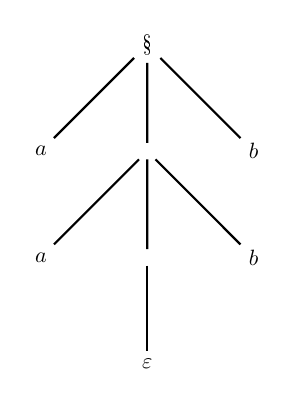
\begin{tikzpicture}   %创建环境
		[thick,scale=0.9, every node/.style={scale=0.8}]
		%thick,scale是整张树形图的大小,可以在0~1内调整树形图的大小
		%every node/.style={scale=0.8}是每个节点文字的大小,可以修改调整节点文字的大小。
		\node {\S}
		child {node {$a$}}
		child {node {\A}
			child {node {$a$}}
			child { node {\A}
				child { node {$\varepsilon$}}
			}
			child {node {$b$}}
		}
		child {node {$b$}};
	\end{tikzpicture}
\end{center}
\end{document}
